En aquest capítol es presenta l'estructura que segueix el codi per resoldre el flux de potències de les xarxes de test. Es concreten les parts que el conformen, la utilitat de cada una i com s'enllacen entre elles. També es fa referència a la forma de les matrius principals que hi intervenen. A causa de la seva simplicitat, no es tracta el codi del circuit de corrent continu ni de la làmpada de descàrrega. És el resultat de replicar directament les equacions.

La Figura \ref{fig:org1} mostra el plantejament del mètode a alt nivell. Aquí s'entra en detall amb la inicialització, amb el càlcul dels coeficients, així com amb l'ajust de la solució a través del mètode de Padé-Weierstrass. Els tres fitxers adjunts que s'especifiquen són els de la Taula \ref{tab:Fitxers}, on es resumeixen les seves funcionalitats.

\begin{table}[!htb]
    \begin{center}
    \begin{tabular}{ll}
    \hline
    Fitxer & Finalitat\\
    \hline
    \hline
    MIH\_propi.py & Inicialització, càlcul de coeficients i solució final\\
    MIH\_original.py & Inicialització, càlcul de coeficients, solució final i P-W\\
    Funcions.py & Padé, Sigma, Thévenin i mètodes recurrents\\
    \hline 
    \end{tabular}
    \caption{Fitxers principals amb les seves funcionalitats}
    \label{tab:Fitxers}
    \end{center}
  \end{table}

El fitxer MIH\_propi.py calcula els coeficients amb la formulació pròpia mentre que el MIH\_original.py ho fa per mitjà de l'altra formulació. Cada un d'ells inicialitza els objectes perquè les matrius d'admitàncies que utilitzen són diferents. Per exemple, el fitxer MIH\_propi.py no fragmenta entre matriu simètrica on les files sumen 0 i asimètrica on això no passa, mentre que el MIH\_original.py sí. L'arxiu Funcions.py és cridat per obtenir la solució final a través dels mètodes recurrents i dels aproximants de Padé. També s'usa a l'hora de calcular els aproximants de Thévenin i els aproximants Sigma.

\section{Inicialització}
La inicialització del programa comença amb la càrrega del fitxer .xlsx de la xarxa a estudiar. Les dades de tots i cada un dels sistemes estudiats es recullen en un d'aquests arxius, que es divideix en dues parts. 

En una pestanya hi ha contingudes les dades de cada bus, que en funció de si és PQ, PV o oscil·lant se sap el seu mòdul de tensió, la fase, la potència activa o la reactiva. En aquesta pestanya també hi apareixen les càrregues d'admitància constant. La seva part real s'anomena shunt re i la imaginària shunt im. Participen en la generació de les matrius d'admitàncies.

A la segona pestanya es defineix la topologia del sistema. Per això, hi ha les dades de les línies i transformadors que enllacen entre busos inicials i busos finals. També s'inclou la relació de transformació (anomenada tap) i el desfasament (angle) que introdueixen. En la majoria dels casos la relació és unitària i el desfasament nul.

Tot plegat comporta que la inicialització sigui tal com es mostra a la Figura \ref{fig:prog0}.

\begin{figure}[!htb] \footnotesize
  \begin{center}
\begin{tikzpicture}[node distance=2.0cm]
  \node (a0) [xshift=0cm]{Fitxer xarxa.xlsx};
  \node (a1) [process, below of = a0, yshift=0.5cm, xshift=-2.75cm] {Lectura de la topologia};
  \node (a2) [process, right of = a1, xshift = 3.5cm] {Lectura dels busos};
  \node (a3) [process, below of = a2, xshift = 0.0cm] {Creació d'índexs de busos};  
  \node (a4) [process, below of = a3, yshift=-0cm] {Definició de vectors V, P i Q};  
  \node (a5) [process, below of = a1, xshift=0cm, yshift = -0.5cm] {Creació de matrius d'admitàncies};
  \node (a6) [below of = a5, yshift=0.5cm] {Ysl, Yred, vec\_shunts,Yslack,};
  \node (a8) [below of = a6, yshift=1.5cm] {Ytapslack, Yseries, Ytap, Yshunts};
  \node (a7) [below of = a4, yshift=0.5cm] {vec\_V, vec\_P, vec\_Q};


  \coordinate (b1) [below of = a1, yshift = -2cm];
  \coordinate (b2) [below of = a2, yshift = 0.5cm];
  \coordinate (b3) [right of = b1];
  \coordinate (b0) [left of = a0, xshift=-2cm];

  \draw[arrow] (a1) -- (a5) node[left, midway] {df\_top};
  \draw[arrow] (a2) -- (a3) node[right, midway] {df\_bus};
  \draw[arrow] (a3) -- (a4) node[right, midway] {sl, pq, pv, pqpv};
  \draw[arrow] (a4) -- (a7) node[left, midway] {};
  \draw[arrow] (-1.4, 0) -|  (a1) node[left, midway] {};
  \draw[arrow] (1.4, 0) -|  (a2) node[left, midway] {};
  \draw (2, -2) --  (2,-2.5) node[left, midway] {};
  \draw (2, -2.5) --  (-2,-2.5) node[above, midway] {df\_bus};
  \draw [arrow] (-2,-2.5) -- (-2, -3.385) node[left, midway] {};
  \draw[arrow] (a5) -- (a6) node[left, midway] {};


  \end{tikzpicture} 
\caption{Esquema d'inicialització dels objectes}
\label{fig:prog0}
\end{center}
\end{figure}

% \begin{figure}[!htb] \footnotesize
%     \begin{center}
%   \begin{tikzpicture}[node distance=2.0cm]
%     \node (a1) [startstop] {Lectura de la topologia};
%     \node (a2) [startstop, right of = a1, xshift = 3.5cm] {Lectura dels busos};
%     \node (a3) [process, below of = a2, xshift = 1cm] {Creació d'índexs de busos};  
%     \node (a4) [process, below of = a3] {Definició de vectors V, P i Q};  
%     \node (a5) [process, below of = a1, xshift=2.5cm, yshift = -1cm] {Definició de matrius d'admitàncies};
%     \coordinate (b1) [below of = a1, yshift = -2cm];
%     \coordinate (b2) [below of = a2, yshift = 0.5cm];
%     \coordinate (b3) [right of = b1];

%     \draw[arrow] (a1) -- (a5) node[left, midway] {};
%     \draw[arrow] (a2) -- (a5) node[left, midway] {};
%     \draw[arrow] (a2) -- (a3) node[left, midway] {};
%     \draw[arrow] (a3) -- (a4) node[left, midway] {};
%     \end{tikzpicture} 
%   \caption{Esquema d'inicialització dels objectes}
%   \label{fig:prog0}
% \end{center}
% \end{figure}

La lectura de les dades dels fitxers .xlsx s'ha dut a terme mitjançant la llibreria Pandas, que es troba programada en Python i serveix per manipular i analitzar estructures de dades. S'ha creat una estructura per a cada pestanya: df\_top per a la topologia i df\_bus per als busos. 

Per tal de treballar amb matrius, en la inicialització i pràcticament en tot el codi s'empra la llibreria NumPy, que s'abrevia com a np. Aquesta integra funcions per adaptar matrius, permet calcular el complex conjugat, dividir una variable en part real i imaginària...

Les matrius d'admitàncies que intervenen a la formulació pròpia són tres: la que conté les branques en sèrie que connecten els busos oscil·lants amb els busos PQ i PV, que s'anomena Ysl; la que compta amb totes les branques en sèrie que veuen els busos PQ i PV, que es coneix pel nom d'Yred; i el vector vec\_shunts, que agrupa les admitàncies degudes a les capacitats del model de les línies així com les càrregues d'impedància constant, totes amb el signe canviat. Equivalen a admitàncies en paral·lel.

La construcció d'Ysl i vec\_shunts s'efectua per observació. Això significa que es recorren totes les files del fitxer per tal de trobar quines admitàncies connecten a cada bus. La creació d'Yred és més metòdica. Parteix de què tots els transformadors compten amb una relació de transformació unitària per llavors emprar:
\begin{equation}
    Y_{serie}=ALA^T\ ,
    \label{eq:incidencia}
\end{equation}
on:

$Y_{serie}$: matriu d'admitàncies de les branques en sèrie amb relacions de transformació unitàries.
\vs
$A$: matriu d'incidència. Compta amb tantes files com busos i tantes columnes com branques hi ha. Les seves entrades són 0, 1 o -1. Defineix entre quins busos enllacen les branques.
\vs
$L$: matriu diagonal amb les admitàncies de les branques en sèrie.

La matriu $Y_{serie}$ dóna lloc a Yred després d'afegir la contribució dels transformadors de relació variable per observació.

A la formulació original entren en joc cinc matrius d'admitàncies. Per un costat la matriu d'admitàncies de les branques en sèrie es divideix en dues: la Yseries i la Ytap. La primera és simètrica perquè fixa totes les relacions de transformació a la unitat, mentre que la Ytap compensa, és a dir, que conté el que falta sumar a Yseries per generar la matriu d'admitàncies total de les branques en sèrie.

Les admitàncies en sèrie que connecten amb el bus oscil·lant també es fragmenten en dos: Yslack i Ytapslack. A la primera s'ha suposat que totes les relacions de transformació són unitàries i la segona serveix per compensar. Finalment, el vector vec\_shunts s'anomena Yshunts en aquesta formulació. Els seus signes no estan girats. 

A la Taula \ref{tab:Fitxersmat} es recullen les matrius d'admitàncies de cada formulació segons el tipus, a manera de resum. Com s'observa, la formulació original utilitza menys matrius d'admitàncies. %En efecte, és més compacta que l'original.

\begin{table}[!htb]
    \begin{center}
    \begin{tabular}{llll}
    \hline
    Fitxer & Sèrie amb l'oscil·lant & Sèrie entre PQ i PV & Paral·lel\\
    \hline
    \hline
    MIH\_propi.py & Ysl & Yred & vec\_shunts \\
    MIH\_original.py & Yslack, Ytapslack & Yseries, Ytap & Yshunts \\
    \hline 
    \end{tabular}
    \caption{Matrius d'admitàncies segons el tipus i el fitxer}
    \label{tab:Fitxersmat}
    \end{center}
  \end{table}

Per altra banda, és necessari emmagatzemar els índexs dels busos en funció de quin tipus es tractin: oscil·lants, PQ o PV. Els vectors que els guarden són respectivament sl, pq i pv. Els dos últims conformen el vector pqpv, que agrupa els índexs dels busos PQ i PV. No obstant això, durant el càlcul de coeficients de les sèries, els busos oscil·lants són dades. Així doncs, no tots els índexs de pqpv són consecutius, el que més endavant complicaria el càlcul. 

Per fer que sí que siguin consecutius, pq es converteix en pq\_, pv en pv\_ i pqpv en pqpv\_. Això s'aconsegueix a partir d'ocupar l'índex del bus o dels busos oscil·lants pels índexs de busos PQ i/o PV.  

Pel que fa als vectors de dades com la tensió, la potència activa o la potència reactiva, es llegeixen de la pestanya de busos. Cada dada es guarda en un vector diferent, que respectivament són vec\_V, vec\_P i vec\_Q. Com que del bus oscil·lant es coneix la tensió en mòdul i angle, se'l tracta per separat. Aquests vectors de dades utilitzen els índexs sl, pq, pv i pqpv en la seva creació però en la posterior obtenció dels coeficients se seleccionen els elements amb la indexació del tipus pqpv\_. 

Encara que no s'ha representat, totes les potències es multipliquen pel factor de càrrega $\lambda$, que en el codi se li associa la variable factor\_carrega.

\section{Càlcul de coeficients}
El càlcul dels coeficients de les sèries és la part essencial del mètode d'incrustació holomòrfica. Tot i que aquest pas resulta la base del mètode, en un inici s'han de captar les dades del problema, dur a terme les definicions inicials i finalment trobar els errors a partir dels coeficients obtinguts. 

En detall, primer el mètode necessita les matrius d'admitàncies definides a la Taula \ref{tab:Fitxersmat}. En funció de la formulació seran unes o altres. També, requereix que se li passin els índexs consecutius, és a dir, pq\_, pv\_, pqpv\_ i el referent al bus o busos oscil·lants, sl. A més, cal definir la profunditat de les sèries, que se simbolitza per la variable prof. 

Al final es poden utilitzar eines que proporcionen informació valuosa, com els aproximants Sigma pel diagnòstic i els aproximants de Thévenin pels mòduls de tensió. No són obligatoris però sí molt recomanables per conèixer millor el sistema.

En resum, el procediment a alt nivell es plasma a la Figura \ref{fig:prog1}.

\tikzstyle{function} = [circle, minimum width=1.5cm, minimum height=1cm, text width=1.7cm, text centered, draw=black, aspect=1]

\begin{figure}[!htb] \footnotesize
  \begin{center}
\begin{tikzpicture}[node distance=2.0cm]
  \node (a3) {pq\_, pv\_,};
  \node (a32) [below of = a3, yshift=1.5cm] {pqpv\_, sl};
  \node (a1) [right of = a3, xshift = 2.5cm] {Ysl, Yred, vec\_shunts,Yslack,};
  \node (a2) [below of = a1, yshift=1.5cm] {Ytapslack, Yseries, Ytap, Yshunts};
  \node (a4) [right of = a1, xshift=2.5cm] {prof};

  \node (a5) [process, below of = a1, xshift=-0cm, yshift=-0.5cm] {Càlcul de $V(s)$ i $Q(s)$ amb MIH};
  \node (a6) [function, below of = a5, xshift=0cm, yshift=-0.5cm] {Funcions.py};

  \node (a7) [below of = a6, xshift=-2.5cm] {$V(s=1)$, $Q(s=1)$,};
  \node (a77) [below of = a7, yshift=1.5cm] {errors};
  \node (a8) [below of = a6, xshift=-0cm] {Sigma};
  \node (a9) [below of = a6, xshift=2cm] {Thévenin};

  \draw[arrow] (a2) -- (a5) node[left, midway] {};
  \draw (0, -0.8) -- (0, -1.2) node[left, midway] {};
  \draw (0, -1.2) -- (3.7, -1.2) node[left, midway] {};
  \draw[arrow] (3.7, -1.2) -- (3.7, -2) node[left, midway] {};
  \draw (9.0, -0.3) -- (9.0, -1.2) node[left, midway] {};
  \draw (9.0, -1.2) -- (5.3, -1.2) node[left, midway] {};
  \draw[arrow] (5.3, -1.2) -- (5.3, -2) node[left, midway] {};

  \draw[arrow] (a5) -- (a6) node[right, midway] {$V(s)$ i $Q(s)$};

  \draw[arrow] (a6) -- (a7) node[right, midway] {};
  \draw[arrow] (a6) -- (a8) node[right, midway] {};
  \draw[arrow] (a6) -- (a9) node[right, midway] {};

  \end{tikzpicture} 
\caption{Esquema del procés de càlcul del MIH}
\label{fig:prog1}
\end{center}
\end{figure}

% \begin{figure}[!htb] \footnotesize
%     \begin{center}
%   \begin{tikzpicture}[node distance=2.0cm]
%     \node (a1) [startstop] {Captació de dades};
%     \node (a2) [process, below of = a1] {Definició de la profunditat};
%     \node (a3) [process, below of = a2] {Càlcul de termes [0], [1], [2] i [$\geq$3]};
%     \node (a4) [function, below of = a3, xshift = 4cm, yshift=0.5cm] {Funcions.py};
%     \node (a5) [process, below of = a4] {Interpretació de $\sigma$ i Thévenin};
%     \node (a6) [process, left of = a5, xshift = -2cm] {Càlcul d'errors};
%     \draw [arrow] (a1) -- (a2) node[left, midway] {};
%     \draw [arrow] (a2) -- (a3) node[left, midway] {};
%     \draw [arrow] (a3) -- (a4) node[left, midway] {};
%     \draw [arrow] (a4) -- (a5) node[left, midway] {};
%     \draw [arrow] (a4) -- (a6) node[left, midway] {};
%     \end{tikzpicture} 
%   \caption{Esquema del procés de càlcul del mètode}
%   \label{fig:prog1}
% \end{center}
% \end{figure}

És molt important establir una profunditat adient, o sigui, un nombre de coeficients suficient per extreure solucions amb poc error però no exagerat per reduir el temps de càlcul. Es podria adoptar l'enfocament de calcular a cada pas l'error, decidir si fa falta calcular el següent coeficient, i així successivament. Tanmateix, per accelerar les simulacions sovint s'opta per concretar una profunditat inicial. Llavors es valora si és adequada en funció de l'error. En principi, com més mal condicionat es troba un sistema, més convé que la profunditat resulti elevada. 

Pel que fa al càlcul de termes, les sèries desconegudes són les tensions dels busos PQ i PV, així com la potència reactiva dels busos PV. Però aquestes no són les úniques sèries, perquè la tensió es divideix en part real i imaginària. També hi intervé la tensió inversa conjugada, que a la vegada es fragmenta en real i imaginària. Així, hi ha un total de 7 tipus de sèries a calcular. Totes elles segueixen l'estructura de la Figura \ref{fig:prog2}.

\begin{figure}[!htb] \footnotesize
    \begin{center}
        \begin{tikzpicture}[scale=0.5]
            \def\a{10}
            \def\b{5}
            \def\c{1}

            \foreach \x in {0,...,\a}
            {   \draw (\x ,0 ) -- (\x ,\b );
                \draw (\x ,\b ) -- (\x ,\b  );
            }
            \foreach \x in {0,...,\b}
            {   \draw (\a ,\x ) -- (\a ,\x );
                \draw (0  ,\x ) -- (\a ,\x );
            }
            % \foreach \x in {0,...,\c}
            % {   \draw (\a ,0  ,\x ) -- (\a ,\b ,\x );
            %     \draw (0  ,\b ,\x ) -- (\a ,\b ,\x );
            % }

            \draw [arrow] (-0.5,5.5) -- (1.5,5.5) node[above, midway] {Busos} ;
            \draw [arrow] (-0.5,5.5) -- (-0.5,3.5) node[left, midway] {Profunditat};
        \end{tikzpicture}
  \caption{Estructura de les matrius de les sèries a calcular}
  \label{fig:prog2}
\end{center}
\end{figure}

A partir de la Figura \ref{fig:prog2} es posa de manifest que a cada tipus de sèrie els coeficients d'un bus ocupen una columna. Aquests busos són els no oscil·lants, és a dir, els PQ i els PV. A la matriu de la sèrie de potència reactiva, les columnes dels busos PQ no s'omplen. El càlcul dels coeficients comença emplenant la primera fila per a totes les sèries, llavors la segona, i així fins que es completen totes. En l'exemplificació de la Figura \ref{fig:prog2} hi hauria 10 busos no oscil·lants amb un total de 5 coeficients cada un. Realment es treballa amb profunditats superiors a aquesta. Es recomanen entre 20 i 40 termes.

La formulació pròpia té la particularitat de retardar el càlcul de la potència reactiva en un pas. Això implica que els primers termes de reactiva es calculen a la mateixa etapa que s'obtenen els segons termes de tensió.

En les dues formulacions es distingeix entre les primeres profunditats i les següents. Per exemple, a la formulació original els primers termes (del tipus $[0]$) corresponen a l'estat de referència. A la formulació pròpia se soluciona un sistema d'equacions nodals relativament simple. En aquesta última formulació es generalitza a partir dels tercers termes, mentre que a la formulació original el fet de dividir les matrius en dues per tal de complir amb l'estat de referència comporta que l'algoritme es generalitzi a partir dels quarts termes. 

El càlcul dels coeficients exigeix resoldre un sistema lineal d'equacions a cada profunditat. En aquest aspecte, el mètode d'incrustació holomòrfica compta amb un avantatge clar davant el mètode de Newton-Raphson, ja que la matriu es manté constant al llarg de totes les profunditats. Per aquest motiu només es factoritza una vegada. La llibreria SciPy conté eines d'àlgebra lineal. Precisament és la que s'utilitza a l'hora de factoritzar la matriu del sistema. 

A més a més, les matrius en forma de blocs que constitueixen la matriu general del sistema són disperses. Per reduir el temps de càlcul es defineixen primer les matrius en forma del tipus coo gràcies a la llibreria SciPy, és a dir, matrius en forma de coordenades. D'aquesta manera només s'emmagatzemen les entrades no nul·les. Per poder factoritzar la matriu del sistema, aquestes matrius de blocs s'acaben convertint al tipus csc, que possibilita la realització d'operacions de forma eficient. 

Tal com es mostra a la Figura \ref{fig:prog1}, quan s'han calculat els coeficients, es criden les funcions de l'arxiu Funcions.py. Aquestes funcions per una banda són els aproximants de Padé i els mètodes recurrents: Delta d'Aitken, transformacions de Shanks, Rho de Wynn, Èpsilon de Wynn, Theta de Brezinski i Eta de Bauer. S'empra la llibreria Numba per reduir els temps de càlcul.  

Totes aquestes funcions avaluen $V(s=1)$ i $Q(s=1)$ per proporcionar els valors de tensió i potència reactiva final. Així es calculen els errors de potència a cada bus i es valora si són acceptables. En cas que no ho fossin s'augmentaria la profunditat o es recorreria al P-W amb la formulació original. Aquesta valoració no s'ha plasmat a la Figura \ref{fig:prog1} amb la idea de mantenir-la simple.

El fitxer Funcions.py també és cridat per obtenir els aproximants Sigma (i conseqüentment el gràfic Sigma), així com per calcular les tensions, tant de la branca estable com de la inestable, amb els aproximants de Thévenin. D'aquesta manera es diagnostica millor el sistema.

\section{Padé-Weierstrass}
El mètode de Padé-Weierstrass resulta l'eina definitiva per afinar la solució del flux de potències quan aquesta es calcula amb la formulació original i l'error és insatisfactori. En un inici parteix de les sèries calculades amb el MIH bàsic, talment, el procés de càlcul dels termes de la Figura \ref{fig:prog1}. A partir d'aquesta informació, que actua com una solució parcial, s'aconsegueix una solució final que en principi minimitza l'error. 

La Figura \ref{fig:prog3} resumeix de forma esquemàtica les etapes per les quals passa i la informació que usa. Tal com s'observa, també es crida el fitxer Funcions.py.

\begin{figure}[!htb] \footnotesize
  \begin{center}
\begin{tikzpicture}[node distance=2.0cm]
  \node (a3) {$V(s)$, $Q(s)$};
  \node (a1) [right of = a3, xshift = 2.5cm] {Ybtildered, Ybtildew};
  \node (a2) [below of = a1, yshift=1.5cm] {Yahatred, Yahatw, Yshunts};
  \node (a4) [right of = a1, xshift=2.5cm] {$s_0$};

  \node (a5) [process, below of = a1, xshift=-0cm, yshift=-0.5cm] {Càlcul de $V'(s')$ i $Q'(s')$ amb P-W};
  \node (a6) [function, below of = a5, xshift=0cm, yshift=-0.5cm] {Funcions.py};

  \node (a7) [below of = a6, xshift=-0cm] {$V(s=1)$, $Q(s=1)$, errors};

  \draw[arrow] (a2) -- (a5) node[left, midway] {};
  \draw (0, -0.3) -- (0, -1.2) node[left, midway] {};
  \draw (0, -1.2) -- (3.7, -1.2) node[left, midway] {};
  \draw[arrow] (3.7, -1.2) -- (3.7, -2) node[left, midway] {};
  \draw (9.0, -0.3) -- (9.0, -1.2) node[left, midway] {};
  \draw (9.0, -1.2) -- (5.3, -1.2) node[left, midway] {};
  \draw[arrow] (5.3, -1.2) -- (5.3, -2) node[left, midway] {};

  \draw[arrow] (a5) -- (a6) node[right, midway] {$V(s)$ i $Q(s)$ finals};

  \draw[arrow] (a6) -- (a7) node[right, midway] {};

  \end{tikzpicture} 
\caption{Esquema del procés que segueix el P-W}
\label{fig:prog3}
\end{center}
\end{figure}

% \begin{figure}[!htb] \footnotesize
%     \begin{center}
%   \begin{tikzpicture}[node distance=2.0cm]
%     \node (a1) [startstop] {Captació de sèries del MIH bàsic};
%     \node (a2) [process, below of = a1] {Definició d'$s_0$};
%     \node (a3) [process, below of = a2] {Càlcul de coeficients amb P-W};
%     \node (a32) [decision, below of = a3] {Fi graons?};
%     \node (a4) [function, right of = a32, xshift = 2.5cm, yshift=0.0cm] {Funcions.py};
%     \node (a5) [process, below of = a4] {Càlcul d'errors};
    
%     \draw [arrow] (a1) -- (a2) node[left, midway] {};
%     \draw [arrow] (a2) -- (a3) node[left, midway] {};
%     \draw [arrow] (a3) -- (a32) node[left, midway] {};
%     \draw [arrow] (a32) -- (a4) node[above, midway] {Sí};
%     \draw [arrow] (a4) -- (a5) node[left, midway] {};
%     \draw (a32) -- (-3, -6) node[above, midway] {No};
%     \draw (-3, -6) -| (-3, -4) node[above, midway] {};
%     \draw [arrow] (-3, -4) -- (a3) node[above, midway] {};

%     \end{tikzpicture} 
%   \caption{Esquema del procés que segueix el P-W}
%   \label{fig:prog3}
% \end{center}
% \end{figure}

Per ser generalitzat, el P-W necessita que els primers coeficients de tensió siguin tots unitaris i els de reactiva nuls. Aleshores, es tracta d'avaluar les sèries inicials de tensió i reactiva a $s_0$. De fet, a la Figura \ref{fig:prog3} $s_0$ s'entén com un vector que agrupa les diverses $s$ a les quals s'avaluen les solucions anteriors. Com s'explica al capítol dedicat al P-W, seleccionar $s_0$ correctament és imprescindible si es vol reduir l'error. No qualsevol valor empetiteix l'error fins a la tolerància establerta.

El vector $s_0$ es calcula amb un mètode d'assaig-i-error. Això significa que primer es treballa amb només un graó. S'avalua si la diferència entre aproximants de Padé consecutius és inferior a la tolerància seleccionada. Si ho és, s'augmenta el valor d'aquell element de $s_0$. Si no ho és, se'l disminueix. Es repeteixen aquestes etapes fins a arribar al límit. Aquest procediment es porta a terme per cada graó.

% Així doncs, la llargada del vector $s_0$ és arbitrària. Cada un dels seus elements en què s'avaluen les sèries anteriors defineix un graó. Per això a la Figura \ref{fig:prog3} es calculen els coeficients fins que no hi ha més graons. Cal dir que al codi s'inclou el càlcul de les diferències entre els valors que proporcionen els aproximants de Padé per ajustar $s_0$. En efecte, la Figura \ref{fig:prog3} es correspon al procés a seguir al final de tot, una vegada $s_0$ ja és conegut.

Durant el càlcul dels coeficients amb el P-W, a part de fragmentar les matrius, es defineixen 7 matrius tridimensionals. Aquestes es corresponen a les tensions (total, part real i part imaginària), a la inversa de les tensions conjugades (total, part real i part imaginària) i a la potència reactiva. Per exemple, la tensió es denota per Up, on p indica que són les noves sèries. La forma d'aquestes matrius es copsa a la Figura \ref{fig:prog4}.

\begin{figure}[!htb] \footnotesize
    \begin{center}
        \begin{tikzpicture}[scale=0.5]
            \def\a{10}
            \def\b{5}
            \def\c{3}

            \foreach \x in {0,...,\a}
            {   \draw (\x ,0  ,\c ) -- (\x ,\b ,\c );
                \draw (\x ,\b ,\c ) -- (\x ,\b ,0  );
            }
            \foreach \x in {0,...,\b}
            {   \draw (\a ,\x ,\c ) -- (\a ,\x ,0  );
                \draw (0  ,\x ,\c ) -- (\a ,\x ,\c );
            }
            \foreach \x in {0,...,\c}
            {   \draw (\a ,0  ,\x ) -- (\a ,\b ,\x );
                \draw (0  ,\b ,\x ) -- (\a ,\b ,\x );
            }

            \draw [arrow] (-4,3.85) -- (-2,3.85) node[below, near end] {Busos} ;
            \draw [arrow] (-4,3.85) -- (-4,1.85) node[left, midway] {Profunditat};
            \draw [arrow] (-4,3.85) -- (-2.5858, 5.4358) node[left, midway] {Graons};
        \end{tikzpicture}
  \caption{Estructura de les matrius de les noves sèries del P-W}
  \label{fig:prog4}
\end{center}
\end{figure}

En el P-W també s'escull una profunditat arbitrària, que per conveniència sovint es fixa a la mateixa que la del mètode d'incrustació holomòrfica bàsic. Com s'observa, l'estructura de la matriu de la Figura \ref{fig:prog4} és idèntica a la de la Figura \ref{fig:prog2} amb la diferència que aquest cop s'afegeix una tercera dimensió, ja que també recull els coeficients per a cada graó. A l'exemple de la Figura \ref{fig:prog4} hi ha 10 busos amb una profunditat de 5 coeficients i 3 graons. Per omplir aquesta matriu, primer s'emplena fila a fila el primer graó, llavors el segon, i així fins que s'acaben. 

Com que el P-W es basa a emprar les sèries anteriorment obtingudes per avaluar-les a $s_0$ i tractar-les com a solucions parcials, es defineixen uns altres dos objectes rellevants. Són les matrius que agrupen les solucions parcials de tensió (Us0) i de potència reactiva (Qs0). La seva forma es plasma a la Figura \ref{fig:prog5}.

\begin{figure}[!htb] \footnotesize
  \begin{center}
      \begin{tikzpicture}[scale=0.5]
          \def\a{3}
          \def\b{10}
          \def\c{1}

          \foreach \x in {0,...,\a}
          {   \draw (\x ,0 ) -- (\x ,\b );
              \draw (\x ,\b ) -- (\x ,\b  );
          }
          \foreach \x in {0,...,\b}
          {   \draw (\a ,\x ) -- (\a ,\x );
              \draw (0  ,\x ) -- (\a ,\x );
          }
          % \foreach \x in {0,...,\c}
          % {   \draw (\a ,0  ,\x ) -- (\a ,\b ,\x );
          %     \draw (0  ,\b ,\x ) -- (\a ,\b ,\x );
          % }

          \draw [arrow] (-0.5,10.5) -- (1.5,10.5) node[above, midway] {Graons} ;
          \draw [arrow] (-0.5,10.5) -- (-0.5,8.5) node[left, midway] {Busos};
      \end{tikzpicture}
\caption{Estructura de les matrius de les solucions parcials}
\label{fig:prog5}
\end{center}
\end{figure}

Tal com es desprèn de la Figura \ref{fig:prog5}, en aquest exemple també es treballa amb 10 busos i 3 graons. És clar, no hi ha una dimensió dedicada a la profunditat perquè es recullen les solucions parcials avaluades a $s_0$, i no els termes que permeten arribar a aquesta solució.

La Figura \ref{fig:prog3} il·lustra que quan s'han calculat tots els coeficients dels graons, és moment de cridar el fitxer Funcions.py. En aquest cas no s'aprofita per calcular els resultats finals amb els mètodes recurrents, obtenir els aproximants Sigma i els de Thévenin, sinó que només es busca avaluar l'última sèrie a $s=1$. Per fer-ho, es podrien utilitzar els mètodes recurrents però la teoria del P-W es basa en els aproximants de Padé.

Finalment, en conèixer les tensions i potències reactives de l'últim graó avaluades a 1, s'efectua el producte d'aquestes per totes les respectives sèries anteriors i s'avalua l'error. En cas que l'error resulti inacceptable, es defineix un altre vector $s_0$ o es varia la profunditat.

Al codi del P-W hi ha quatre matrius d'admitàncies rellevants. Aquestes són Yahatred, Yahatw, Ybtildred, Ybtildew. Les dues primeres corresponen a parts de la matriu $\widehat{Y}^{(a)}$. En concret, Yahatw conté les connexions amb el bus oscil·lant, mentre que Yahatred agrupa els elements per a la resta de busos, és a dir, els PQ i PV. Per la seva banda, Ybtildew representa els elements del tipus $\widetilde{Y}^{(b)}_{iw}$. Ybtildered és la matriu on les files sumen 0 reduïda als busos PQ i PV, que es denota per $\widetilde{Y}^{(b,red)}$. 
Aquestes matrius es resumeixen a la Taula \ref{tab:Fitxersmat2}.

\begin{table}[!htb]
  \begin{center}
  \begin{tabular}{lll}
  \hline
  Tipus & Enllaça PQ i PV & Enllaça l'oscil·lant\\
  \hline
  \hline
  Compleix amb l'estat de referència & Ybtildred & Ybtildew \\
  No compleix amb l'estat de referència & Yahatred & Yahatw \\
  \hline 
  \end{tabular}
  \caption{Matrius d'admitàncies del programa del P-W segons els busos que considera i el tipus}
  \label{tab:Fitxersmat2}
  \end{center}
\end{table}

\section{Incorporació al GridCal}
Una part del codi en què es basa aquest treball s'ha integrat a la plataforma GridCal. GridCal és un programari de codi obert utilitzat per a temes de recerca i consultoria relacionada amb sistemes elèctrics de potència des de l'any 2015. Està concebut per permetre que sigui extensible segons les necessitats dels usuaris, i a més, inclou una interfície gràfica. Igual que el codi desenvolupat en aquest treball, es troba escrit en Python.

L'autor del projecte va posar-se en contacte amb Santiago Peñate, el creador del GridCal, per comunicar-li que havia generat un codi capaç de resoldre el flux de potències amb el mètode d'incrustació holomòrfica, tant si hi havia busos PQ com PV. Posteriorment aquest codi es va incorporar a la versió 3.7.0 del GridCal. 

Segons Peñate (2020a), és sensat afirmar que aquest és el primer programari en codi obert fonamentat en el mètode d'incrustació holomòrfica que soluciona xarxes reals. A la Figura \ref{fig:solversGridCal} apareixen els diversos mètodes resolutius del flux de potències de la versió 3.7.0 del GridCal, amb el mètode d'incrustació holomòrfica ressaltat.

\begin{figure}[!htb] \footnotesize
  \begin{center}
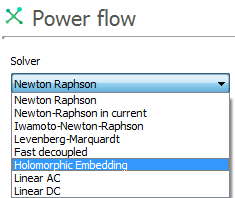
\includegraphics[scale=1.0]{Inputs/solvers2}
\caption{Mètodes resolutius del flux de potències amb què compta la versió 3.7.0 del GridCal}
\label{fig:solversGridCal}
\end{center}
\end{figure}

La formulació integrada és la formulació pròpia. També s'han inclòs els aproximants Sigma. A l'apartat de treballs futurs de les conclusions es contemplen altres funcionalitats a incorporar.

